
%% ESTA PARTE ES PARA EXPLICAR EL SUMMIT

\section{Managing a real robot: Summit XL}
\begin{frame}{Summit XL}
\begin{figure}
    \centering
    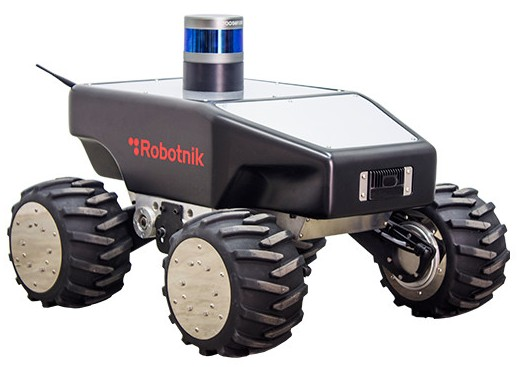
\includegraphics[scale=0.5]{img/ros/summit-xl.jpg}
\end{figure}
\end{frame}

\subsection{Summit Installation}
\label{subsec:summit_installation}

\begin{frame}[fragile]{PC installation}
\begin{enumerate}
    \item Install ROS noetic on PC or use a Docker image.
    \item Network configuration:
    \begin{itemize}
        \item Connect to the router of the robot (SSID: SUMMIT)
        \item Add to the /etc/hosts file the following data:
\begin{lstlisting}[language=shell]
192.168.0.200   shl00-230623aa
\end{lstlisting}
        \item Configure ROS\_MASTER and ROS\_IP parameters:
\begin{lstlisting}[language=shell]
export ROS_MASTER_URI=http://shl00-230623aa:11311
export ROS_IP=<IP provided by the router of the robot>
\end{lstlisting}
    
    \end{itemize}
\end{enumerate}
\end{frame}

\subsection{Summit Simulation}

\begin{frame}[fragile]{Summit Simulation in PC}
Install the repository of Robotnik in the workspace:
\begin{lstlisting}[language=shell]
$ cd catkin_ws
$ sudo apt-get install -y python3-vcstool
$ vcs import --input https://raw.githubusercontent.com/RobotnikAutomation/summit_xl_sim/noetic-devel/repos/summit_xl_sim_devel.repos
$ rosdep install --from-paths src --ignore-src --skip-keys="summit_xl_robot_control marker_mapping robotnik_locator robotnik_pose_filter robotnik_gazebo_elevator" -y -r
$ catkin_make
$ source devel/setup.bash
\end{lstlisting}

Launch the simulation:
\begin{lstlisting}[language=shell]
$ roslaunch summit_xl_sim_bringup summit_xl_complete.launch
\end{lstlisting}
\end{frame}

\begin{frame}[fragile]{Summit Simulation with docker}

Robotnik provides in their repository a docker image with all the software needed.

\begin{lstlisting}[language=shell]
$ git clone https://github.com/RobotnikAutomation/summit_xl_sim.git
$ cd summit_xl_sim
$ git checkout melodic-devel
$ cd docker/
$ export ROS_BU_PKG="summit_xl_sim_bringup"
$ export ROS_BU_LAUNCH="summit_xl_complete.launch"
$ nvidia-smi &>/dev/null \
  ln -sf docker-compose-nvidia.yml docker-compose.yml \
  || ln -sf docker-compose-intel.yml docker-compose.yml
$ docker compose up
\end{lstlisting}

To connect to a terminal in the container you can launch:
\begin{lstlisting}[language=shell]
$ docker exec -it docker-base-1 /bin/bash
\end{lstlisting}
\end{frame}


\section{Speech recognition}

\begin{frame}[fragile, allowframebreaks]{Getting started with speech recognition}

Prerequisites:
\begin{lstlisting}[language=shell]
$ sudo apt install python-pip
$ sudo pip install pyaudio
$ sudo pip install SpeechRecognition
\end{lstlisting}

A first example:
\begin{lstlisting}[language=python]
#!/usr/bin/env python
# -*- coding: utf-8 -*

import speech_recognition as sr

def listen():
    r = sr.Recognizer()
    m = sr.Microphone()

    while True:
        with m as source:
            r.adjust_for_ambient_noise(source)
            print("Say something!")
            try:
                audio = r.listen(source, timeout=1, phrase_time_limit=10)
                print("Got it! Now to recognize it...")
            except sr.WaitTimeoutError:
                pass

        try:
            value = r.recognize_google(audio)#, language="hu-HU")
            print("You said '%s'" % value)
        except sr.UnknownValueError:
            print("Oops! Didn't catch that")
        except sr.RequestError as e:
            print("Oops! Couldn't request results from Google Speech Recognition service; {0}".format(e))

if __name__ == '__main__':
    listen()
\end{lstlisting}

\end{frame}


\section{Arduino and ROS}

\begin{frame}[fragile, allowframebreaks]{Getting started with Arduino and ROS}

\href{http://wiki.ros.org/rosserial_arduino/Tutorials}{Link Tutoriales ROS y Arduino}.

Install rosserial package:
\begin{lstlisting}[language=shell]
$ sudo apt install ros-noetic-rosserial
\end{lstlisting}

Install in the Arduino IDE the latest version of the Rosserial Arduino Library by Joshua Frank.
\begin{lstlisting}[language=shell]
Sketch > Manage Library > Include Library > Manage Libraries
\end{lstlisting}

A first \href{https://microcontrollerslab.com/ros-arduino-rosserial-publish-range-hc-sr04-ultrasonic/}{example} for ultrasonic sensor:
\begin{lstlisting}[language=c]
#include <ros.h>
#include <ros/time.h>
#include <sensor_msgs/Range.h>
#define USE_USBCON

ros::NodeHandle  nh;
sensor_msgs::Range range_msg;
ros::Publisher pub_range( "/ultrasound", &range_msg);

int trigger_pin = 9;
int echo_pin = 12;


long range_time;
char frameid[] = "/ultrasound";


void setup() {
  nh.initNode();
  nh.advertise(pub_range);
  range_msg.radiation_type = sensor_msgs::Range::ULTRASOUND;
  range_msg.header.frame_id =  frameid;
  range_msg.field_of_view = 0.1;  
  range_msg.min_range = 0.0;
  range_msg.max_range = 6.47;
}

void loop()
{
  if ( millis() >= range_time ){ 
      range_msg.range = getRange() / 100;
      range_msg.header.stamp = nh.now();
      pub_range.publish(&range_msg);
      range_time =  millis() + 50;
    }    
    nh.spinOnce();
}

long microsecondsToCentimeters(long microseconds)
{
// The speed of sound is 340 m/s or 29 microseconds per centimeter.
// The ping travels out and back, so to find the distance of the
// object we take half of the distance travelled.
return microseconds / 29.1 / 2;
}

float getRange()
{
  long duration;
  
  // PING is triggered by a HIGH pulse of 2 or more microseconds.
  // Give a short LOW pulse beforehand to ensure a clean HIGH pulse:
  pinMode(trigger_pin, OUTPUT);
  digitalWrite(trigger_pin, LOW);
  delayMicroseconds(2);
  digitalWrite(trigger_pin, HIGH);
  delayMicroseconds(10);
  digitalWrite(trigger_pin, LOW);
  
  // The same pin is used to read the signal from the PING))): a HIGH
  // pulse whose duration is the time (in microseconds) from the sending
  // of the ping to the reception of its echo off of an object.
  pinMode(echo_pin, INPUT);
  duration = pulseIn(echo_pin, HIGH);
  
  // convert the time into a distance
  return microsecondsToCentimeters(duration);
}
\end{lstlisting}

\end{frame}
\section{Autonomous navigation}
\subsection{SLAM Map Building with Summit XL}

\begin{frame}[fragile]{SLAM with Summit XL}
The SLAM (Simultaneous Localization and Mapping) is a technique to draw a map by estimating current location in an arbitrary space. Steps: %The SLAM is a well-known feature of TurtleBot from its predecessors. \href{https://youtu.be/lkW4-dG2BCY}{
\includegraphics[height=.3cm]{./img/link.png}}

\begin{enumerate}
    \item Launch the docker container:
\begin{lstlisting}[language=shell]
$ rocker --x11 --network host --privilege --name ros-noetic --volume <path_to_shared_folder>:/root/catkin_ws -- docker.io/osrf/ros:noetic-desktop-full
\end{lstlisting}
    \item Configuration inside the container and launch Rviz:
\begin{lstlisting}[language=shell]
$ export ROS_MASTER_URI=http://shl00-230623aa:11311
$ export ROS_IP=<IP provided by the router of the robot>
$ rviz
\end{lstlisting}
    \item Connect to the robot in another terminal and launch the mapping functionality:
\begin{lstlisting}[language=shell]
$ ssh robot@shl00-230623aa
$ roslaunch summit_xl_localization slam_gmapping.launch scan_topic:=/robot/top_3d_laser/scan
\end{lstlisting}
    \item Move the robot to create the map and save it inside the robot:
\begin{lstlisting}[language=shell]
$ ssh robot@shl00-230623aa
$ cd /home/robot/EMPOTRADAS
$ mkdir mapa_<name>
$ rosrun map_server map_saver -f /home/robot/EMPOTRADAS/mapa_<name>/mapa_<name>
\end{lstlisting}
\end{enumerate}
\end{frame}


% \vspace{.1cm}
% Launch Gazebo:
% \begin{lstlisting}[language=shell]
% $ roslaunch turtlebot3_gazebo turtlebot3_world.launch
% \end{lstlisting}

% Launch SLAM:
% \begin{lstlisting}[language=shell]
% $ roslaunch turtlebot3_slam turtlebot3_slam.launch slam_methods:=gmapping
% \end{lstlisting}

% Remotely Control TurtleBot3:
% \begin{lstlisting}[language=shell]
% $ roslaunch turtlebot3_teleop turtlebot3_teleop_key.launch
% \end{lstlisting}

% Save the Map:
% \begin{lstlisting}[language=shell]
% $ rosrun map_server map_saver -f ~/map
% \end{lstlisting}


\begin{frame}[fragile]{Navigation with Summit XL}
For navigation with Summit XL follow the next steps: 
\begin{enumerate}
    \item Open a terminal inside the robot and launch the localization:
\begin{lstlisting}[language=shell]
$ ssh robot@shl00-230623aa
$ roslaunch summit_xl_localization localization_complete.launch maps_path:=/home/robot/EMPOTRADAS/ map_file:=mapa_<name>/mapa_<name>.yaml scan_topic:=/robot/top_3d_laser/scan id_robot:=robot
\end{lstlisting}

    \item Open other terminal inside the robot and launch the navigation:
\begin{lstlisting}[language=shell]
$ ssh robot@shl00-230623aa
$ roslaunch robot_bringup navigation_complete.launch 
\end{lstlisting}
    
    \item In the container launch Rviz to see the status of the robot:
\begin{lstlisting}[language=shell]
$ rviz
\end{lstlisting}

\item Configuration in Rviz:
\begin{itemize}
    \item $2D Pose Estimate > "right click" > Tool Properties > Topic > "/robot/initialpose"$
    \item $2D Nav Goal > "right click" > Tool Properties > Topic > "/robot/move\_base\_simple/goal"$
\end{itemize}
\end{enumerate}
\end{frame}


\begin{frame}[fragile, allowframebreaks]{Create a node to send a goal}


A first \href{http://wiki.ros.org/navigation/Tutorials/SendingSimpleGoals}{example}:
\begin{lstlisting}[language=c]
#include <ros/ros.h>
#include <move_base_msgs/MoveBaseAction.h>
#include <actionlib/client/simple_action_client.h>

typedef actionlib::SimpleActionClient<move_base_msgs::MoveBaseAction> MoveBaseClient;

int main(int argc, char** argv){
  ros::init(argc, argv, "simple_navigation_goals");

  //tell the action client that we want to spin a thread by default
  MoveBaseClient ac("move_base", true);

  //wait for the action server to come up
  while(!ac.waitForServer(ros::Duration(5.0))){
    ROS_INFO("Waiting for the move_base action server to come up");
  }

  move_base_msgs::MoveBaseGoal goal;

  //we'll send a goal to the robot to move 1 meter forward
  goal.target_pose.header.frame_id = "base_link";
  goal.target_pose.header.stamp = ros::Time::now();

  goal.target_pose.pose.position.x = 1.0;
  goal.target_pose.pose.orientation.w = 1.0;

  ROS_INFO("Sending goal");
  ac.sendGoal(goal);

  ac.waitForResult();

  if(ac.getState() == actionlib::SimpleClientGoalState::SUCCEEDED)
    ROS_INFO("Hooray, the base moved 1 meter forward");
  else
    ROS_INFO("The base failed to move forward 1 meter for some reason");

  return 0;
}
\end{lstlisting}

\end{frame}


% \begin{frame}[fragile]{Virtual Navigation with Summit XL}
% For virtual Navigation in Gazebo, instead of running the actual robot, you can select the various environments and robot models mentioned above, and the Navigation-related commands.

% \vspace{.1cm}
% Execute Gazebo:
% \begin{lstlisting}[language=shell]
% $ roslaunch turtlebot3_gazebo turtlebot3_world.launch
% \end{lstlisting}

% Execute Navigation:
% \begin{lstlisting}[language=shell]
% $ roslaunch turtlebot3_navigation turtlebot3_navigation.launch map_file:=$HOME/map.yaml
% \end{lstlisting}
% \end{frame}

\section{RaspberryPi Installation and Configuration}
\begin{frame}[fragile, allowframebreaks]{RaspberryPi Installation and Configuration}
To install Ubuntu Server 20.04.5 LTS in the Raspberry Pi and Configure it to connect with Summit you need to follow the next steps:

\begin{enumerate}
    \item Intall Raspberry Pi Imager:
\begin{lstlisting}[language=shell]
$ sudo snap install rpi-imager
\end{lstlisting}
    \item Connect a MicroSD card to your Computer and follow the next step in the graphical interface.
\begin{lstlisting}[language=shell]
Choose OS > Other general-purpose SO > Ubuntu > Ubuntu Server 20.04.5 LTS (64 bits)
Choose Storage > Select the MicroSD card
Write
\end{lstlisting}
    \item Plug the card into the Raspberry Pi and connect: keyboard, ethernet and HDMI:
\begin{lstlisting}[language=shell]
user: ubuntu
pass: ubuntu
(The first login is necessary to change the password (f.e.:ubunturaspy)
\end{lstlisting}
    \item Configure the Layout of the keyboard in Spanish: 
\begin{lstlisting}[language=shell]
$ sudo apt-get install console-data
\end{lstlisting}
    \item Configure the Wi-Fi Connection to Summit XL:
\begin{lstlisting}[language=shell]
$ sudo apt install network-manager
$ nmtui
Select "Activate a connection"
Select the wifi of Summit (SUMMIT)
\end{lstlisting}
    \item Configure the connection to Summit:
\begin{lstlisting}[language=shell]
$ ssh ubuntu@<IP>
$ sudo nano /etc/hosts
(Add)
192.168.0.200   shl00-230623aa
$ nano .bashrc
(Add to the final of the file)
source /opt/ros/noetic/setup.bash
ROS_MASTER_URI=http://shl00-230623aa:11311
ROS_IP=<IP>
$ source bashrc
$ rostopic list
...
\end{lstlisting}    

\end{enumerate}
\end{frame}
